\newpage
\section{Chapter 2}

\begin{figure}[H]
	\centering
	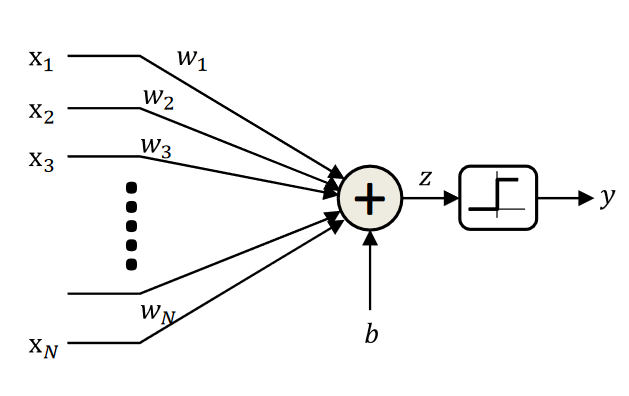
\includegraphics[width=0.5\textwidth]{2_perceptron}
\end{figure}

\hfill\break
Each individual neurons can be represented as a threshold unit.
\begin{itemize}
	\item It fires if the affine function of inputs is positive.
	\item The bias value is the negative of threshold $T$.
\end{itemize} 

\begin{align*}
	z &= \sum_{i}w_ix_i + b \\
	y &= 
\begin{cases} 
	1, & \text{if } z \geq 0 \\
	0, & \text{else }
\end{cases}
\end{align*}

\hfill\break
Once we can represent the neuron in this manner, we can modify the activation threshold function to something different such as:
\begin{itemize}
	\item We define \textbf{activation function} as the function that acts on the weighted combination of inputs and bias.
	 
\end{itemize}
\paragraph{Soft Perceptron (Logistic)}
A squashing function instead of a threshold at the output. This way the output goes rather smooth from $0$ to $1$.
\begin{align*}
	z &= \sum_{i}w_ix_i + b \\
	y &= \frac{1}{1 + \exp (-z)}
\end{align*}

\hfill\break
We can also replace the activation function with other mathematical function such as $\tanh$, $\text{softplus}$ and $\text{rectifier}$.

\subsection{Multi-layer Perceptron}
MLP is a network of perceptrons as the perceptrons of current layer are fed to other perceptrons on the next layer.

\paragraph{Deep Structures}
In any directed graph with input source nodes and output sink nodes, ``depth'' is the length of the longest path from a source to a sink.
\begin{itemize}
	\item A ``source'' node in a directed graph is a node that has only outgoing edges.
	\item A ``sink'' node is a node that has only incoming edges.
\end{itemize}

\hfill\break
This is an example of depth 2 graph.
\begin{figure}[H]
	\centering
	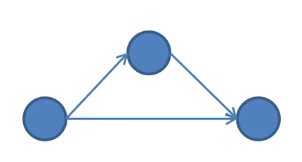
\includegraphics[width=0.4\textwidth]{2_2depth}
\end{figure}

\hfill\break
This is an example of depth 3 graph.
\begin{figure}[H]
	\centering
	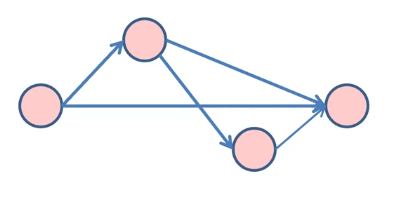
\includegraphics[width=0.4\textwidth]{2_3depth}
\end{figure}

\hfill\break
In multilayer perceptron, a network is considered ``deep'' if the depth of the output neurons is greater than $2$.

\subsection{Layer}
Layer is a set of neurons that are all at the same depth  with respect to the input (sink). This would imply that the ``depth'' of the layer is the depth of the neurons in the layer with respect to the input.

\begin{figure}[H]
	\centering
	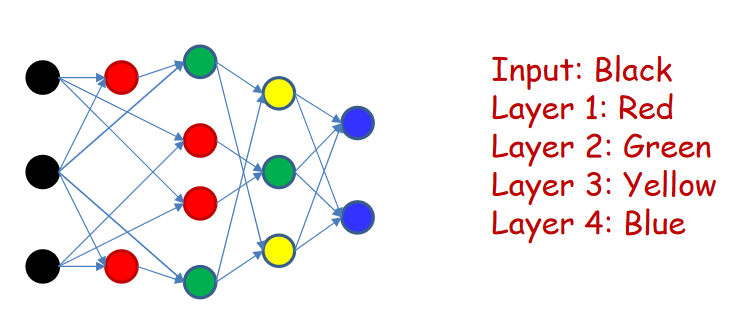
\includegraphics[width=0.75\textwidth]{2_layer}
\end{figure}

\hfill\break
In multi-layered perceptron:
\begin{itemize}
	\item Inputs are real or Boolean stimuli.
	\item Outputs are real or Boolean values.
	\item It can compose both Boolean and real-valued functions.
	\item We can have multiple outputs for a single input.
\end{itemize}

\subsection{MLP as universal Boolean functions.}
We are already aware with perceptron capability as a Boolean gate as it can model any simple binary Boolean gate (OR, AND \& NOT).

\begin{figure}[H]
	\centering
	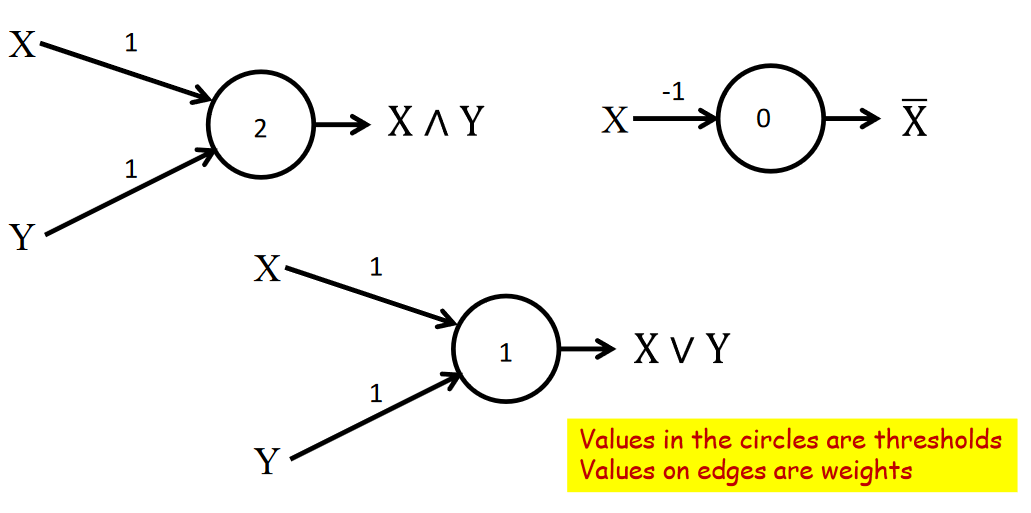
\includegraphics[width=\textwidth]{2_boolean_gate}
\end{figure}

\begin{itemize}
	\item For the AND gate, the boundary condition is $X + Y \geq 2$
	\item For the OR gate, the boundary condition is $X + Y \geq 1$
	\item For the NOT gate, the boundary condition is $-X \geq 0$
\end{itemize}

\hfill\break
It also enables us to compose a much more complex network, for example a universal AND gate where the network is only fired if every input fed to the network is true.

\paragraph{Universal AND Gate}

\begin{figure}[H]
	\centering
	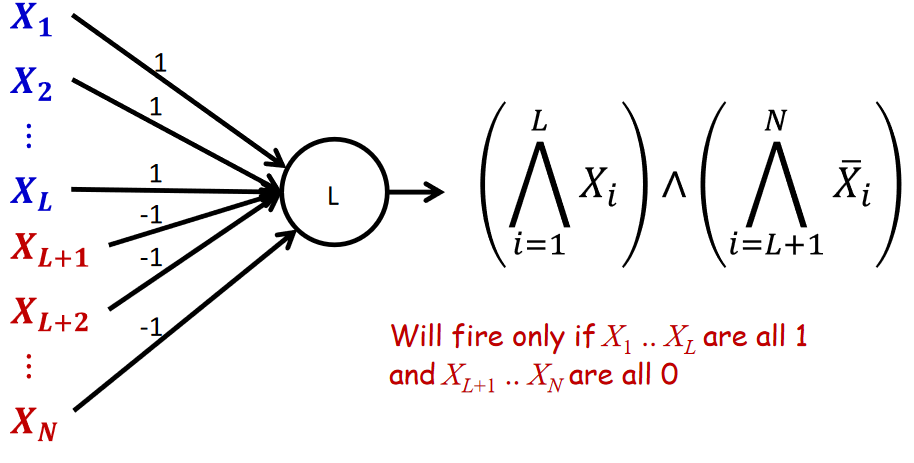
\includegraphics[width=0.5\textwidth]{2_universal_and}
\end{figure}

Suppose that $X_1,X_2,...,X_L$ has weight value of $1$ and $X_{L+1},X_{L+2},...,X_N$ has weight value of $-1$, the condition for the perceptron to fire has to be:
\begin{align}
	(X_1+X_2+...+X_L) - (X_{L+1},X_{L+2},...,X_N) \geq L
\end{align}

\paragraph{Universal OR Gate}

\begin{figure}[H]
	\centering
	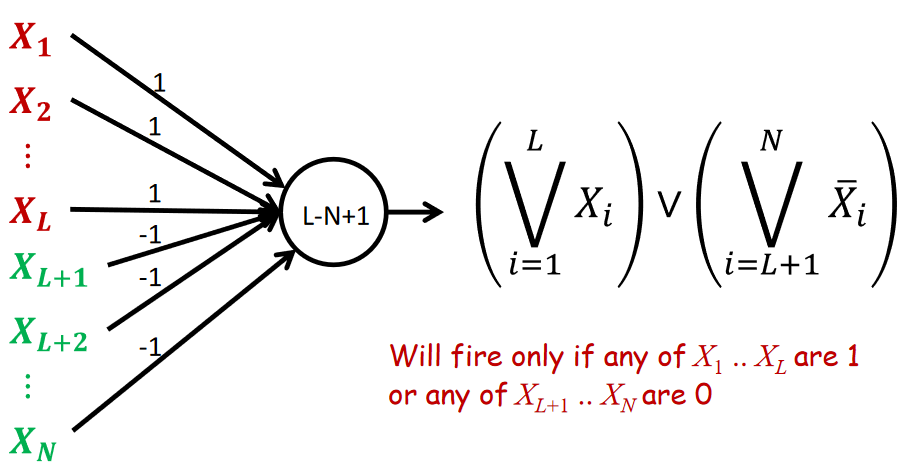
\includegraphics[width=0.5\textwidth]{2_universal_or}
\end{figure}

Suppose that $X_1,X_2,...,X_L$ has weight value of $1$ and $X_{L+1},X_{L+2},...,X_N$ has weight value of $-1$, the condition for the perceptron to fire has to be if any value of the first set is $1$ or any value from the second set is $0$:
\begin{align}
	(X_1+X_2+...+X_L) - (X_{L+1},X_{L+2},...,X_N) \geq L - N + 1
\end{align}

\paragraph{Generalized Majority Gate}

\begin{figure}[H]
	\centering
	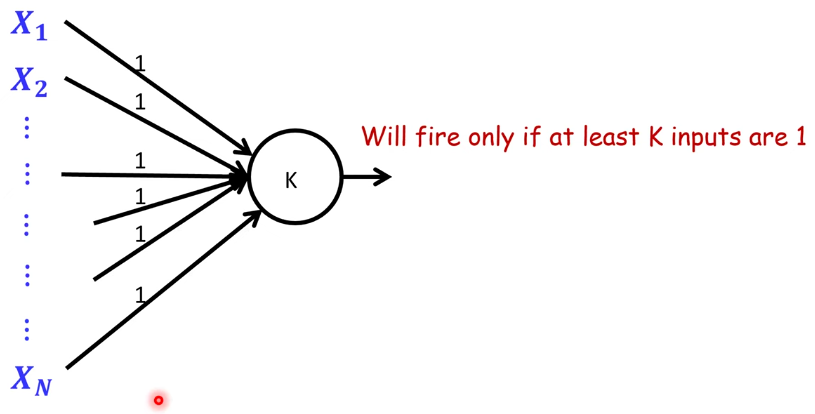
\includegraphics[width=0.5\textwidth]{2_majority_gate}
\end{figure}

\hfill\break
Due to perceptrons being able to model Boolean functions, they able to model complex things that are made of Boolean functions. This also means that for any odd Boolean function, wee can construct a multi-layerr perceptron that can compute this Boolean function. This is what is meant by MLPs being a universal Boolean functions. For any Boolean functions, regardless of their complexity, we can compose an MLP that will compute said function. This lead to a new question, how many layers will they need to be sufficient at modeling said Boolean function? What is the smallest number of layers will be required?


\hfill\break
Any Booleans function can be represented by a truth table. For example:


\begin{table}[H]
	\centering
	\begin{tabular}{|c|c|c|c|c|c|}
			\hline
			$X_1$    & $X_2$     & $X_3$    & $X_4$    & $X_5$    & $Y$   \\
			\hline
			0        & 0        & 1        & 1        & 0        & 1     \\
			0        & 1        & 0        & 1        & 1        & 1     \\
			0        & 1        & 1        & 0        & 0        & 1     \\
			1        & 0        & 0        & 0        & 1        & 1     \\
			1        & 0        & 1        & 1        & 1        & 1     \\
			1        & 1        & 0        & 0        & 1        & 1     \\
			\hline
	\end{tabular}
\end{table}

\hfill\break
In order to get a Boolean function that represent this table, we only have to list the portion of the table that corresponds to the output 1. We can write it as disjunctive normal formula for this table. 

\begin{align}
	Y = \bar{X_1}\bar{X_2}X_3X_4\bar{X_5} + \bar{X_1}X_2\bar{X_3}X_4X_5 + \bar{X_1}X_2X_3\bar{X_4}\bar{X_5} +\\ X_1\bar{X_2}\bar{X_3}\bar{X_4}X_5 + X_1\bar{X_2}X_3X_4X_5 + X_1X_2\bar{X_3}\bar{X_4}X_5
\end{align}

\hfill\break
Once we have obtained the Boolean function in this manner, we can create an MLP where each of the perceptron is an Universal AND gate. These perceptrons is then combined as Universal OR gate.


\begin{figure}[H]
	\centering
	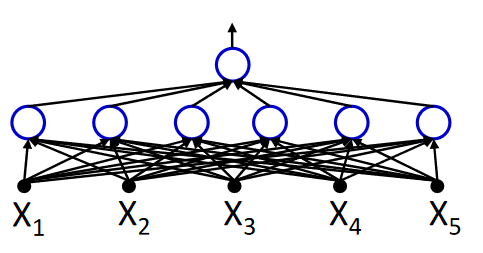
\includegraphics[width=0.5\textwidth]{2_truth_table}
\end{figure}

\hfill\break
This would means that MLP with 1 layer is sufficient enough to model any Boolean Function. This lead to a new question, what is the largest number of perceptrons required in the single hidden layer for an N-input-variable function?

\subsection{Karnaugh Map}
Boolean function can be reduced using Karnaugh Map. It represent a truth table as a grid. Adjacent boxes can be ``grouped'' to reduce the DNF formula for the table.

%\begin{figure}[H]
%\centering
%\begin{Karnaugh}{$v_w$}{$x_y$}
%	\content{0,0,0,0,0,0,0,0,0,0,0,0,0,0,0,0}
%	\implicant{0}{2}{red}
%	\implicant{5}{15}{purple}
%	\implicanttopbottom[3pt]{1}{10}{blue}
%	\implicantcorners[2pt]{orange}
%	\implicantside{4}{14}{green}
%\end{Karnaugh}
%\end{figure}

\begin{figure}[H]
	\centering
	\begin{Karnaugh}{$WX$}{$YZ$}
		\content{1,0,1,0,1,1,0,0,1,0,1,0,1,0,0,0}
		\implicant{4}{5}{red}
		\implicant{0}{8}{blue}
		\implicanttopbottom[3pt]{2}{10}{green}
	\end{Karnaugh}
\end{figure}

\hfill\break
We can group these 3 neighbours together:

\begin{align}
	O = \bar{Y}\bar{Z} + \bar{W}X\bar{Y} + \bar{X}Y\bar{Z}
\end{align}

\begin{itemize}
	\item Regardless value of $W$ and $X$, $Y$ and $Z$ is always $0$.
	\item The function going to fire when $W$ is always $0$ while $X$ can be anything, while $Y$ has to always be $0$.
	\item The other condition for it to fire is when $Y$ is always $1$ while $Z$ is always $0$ and $X$ is always $0$.
\end{itemize}


\hfill\break
Although there are 8 conditions when the network will fire, only 3 perceptions is needed to construct the MLP. The general idea is, when we want to construct the DNF formula, we want to construct it with thee minimum number of clauses.

\begin{figure}[H]
	\centering
	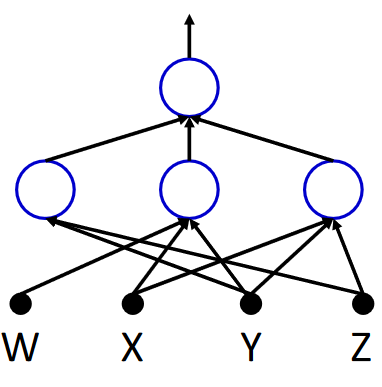
\includegraphics[width=0.5\textwidth]{2_reduced_dnf}
\end{figure}

\hfill\break
On irreducible DNF, the size of required perceptrons in the hidden layer can get exponentially large ($2^{n-1}$).

\begin{figure}[H]
	\centering
	\begin{Karnaugh}{$WX$}{$YZ$}
		\content{1,0,0,1,0,1,1,0,0,1,1,0,1,0,0,1}
	\end{Karnaugh}
\end{figure}

\hfill\break
While the DNF cannot be reduced, this type of Boolean function can still be generalized. Is it possible to reduce the number of units if we use multiple hidden layers?

This checkered pattern is a form of XOR Boolean function which become TRUE only if:
\begin{itemize}
	\item 1 flag is FALSE while the rest of the flags is TRUE.
	\item 1 flag is TRUE while the rest of the flags is FALSE.
\end{itemize}

\begin{align}
	O = W \oplus X \oplus Y \oplus Z
\end{align}

\hfill\break
Since we need 1 hidden layer consisting of 2 perceptrons to construct XOR gate:

\begin{figure}[H]
	\centering
	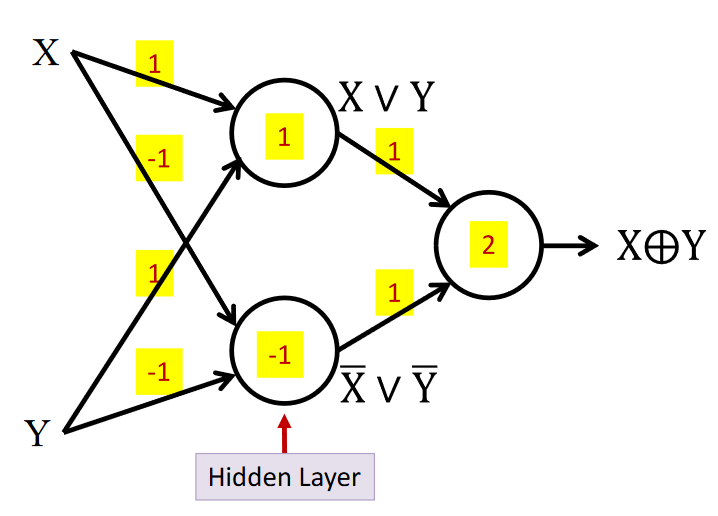
\includegraphics[width=0.5\textwidth]{2_xor}
\end{figure}

\hfill\break
We can cascade the XOR gates to construct the solution for the MLP.

\begin{figure}[H]
	\centering
	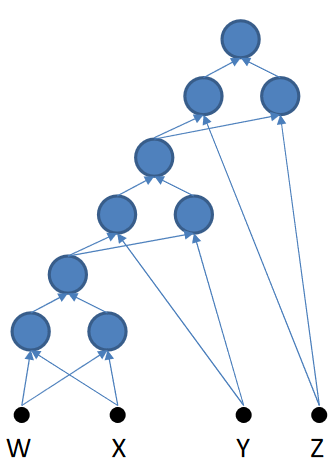
\includegraphics[width=0.5\textwidth]{2_xor_cascade}
\end{figure}

\hfill\break
For cascading XOR gates with 4 parameter, 9 perceptrons would be required to construct the Boolean function MLP. The solution of the cascading XOR gates would be $3\times (N-1)$ number of perceptrons. 

These can be arranged in only $2\log_2(N)$ layers. Suppose that wee have $X_1, X_2, ..., X_N$ number of perception. We can keep pairing terms such as:

\begin{align}
	O &= X_1 \oplus X_2 \oplus X_3 \oplus X_4 \oplus X_5 \oplus X_6 \oplus X_7 \oplus X_8\\
	O &= ((X_1 \oplus X_2) \oplus (X_3 \oplus X_4)) \oplus ((X_5 \oplus X_6) \oplus (X_7 \oplus X_8))
\end{align}

\begin{figure}[H]
	\centering
	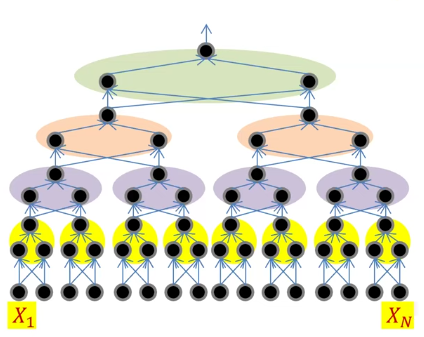
\includegraphics[width=0.75\textwidth]{2_multi_layer_xor}
\end{figure}

\subsection{Implementation of MLP on K-layer.}
Using only K-hidden layers will require $2^{CN}$ neurons in the K-th layer, where

\begin{align}
	C = 2^{-\frac{K-1}{2}}
\end{align}

\begin{figure}[H]
	\centering
	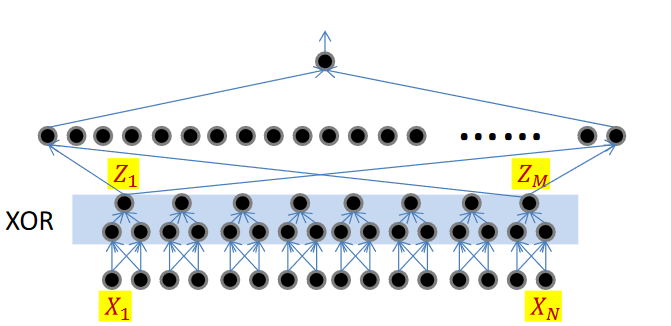
\includegraphics[width=0.75\textwidth]{2_k_layer_xor}
\end{figure}

\hfill\break
Going through the layer until the K-th layer, we keep reducing the number of neutrons by factor of $2$. However, we still have to XOR whatever number of neutrons left on the K-th layer, exponentially increasing the number of neutrons.

\begin{itemize}
	\item Because the output is the XOR for all the $\frac{N}{2^{\frac{K-1}{2}}}$ values output by the K-1-th hidden layer.
	\item In other word, reducing the numbers of layers below the minimum will result in an exponentially sized network to express the function fully.
	\item A network with fewer than minimum required number of neutrons cannot model the function.
\end{itemize}

\subsection{Network Parameters.}
The actual number of parameters in a network is the number of connections. For example, for a network with 1 hidden layer consisting of 5 neutrons, the number of parameters in a network is 30.

\begin{figure}[H]
	\centering
	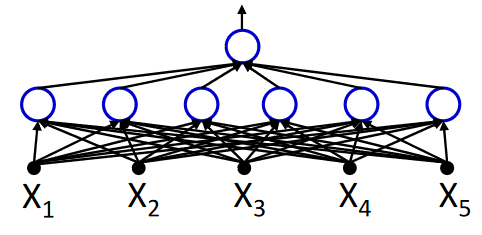
\includegraphics[width=0.75\textwidth]{2_1_layer_mlp}
\end{figure}

This is the number that really matters in software or hardware implementation of the neural networks. Networks that require an exponential number of neurons will require an exponential number of weights.

\subsection{Composing complicated ``decision'' boundary.}
Once we can computes a linear boundary, we can compose more complex decision boundary as shown below.

\begin{figure}[H]
	\centering
	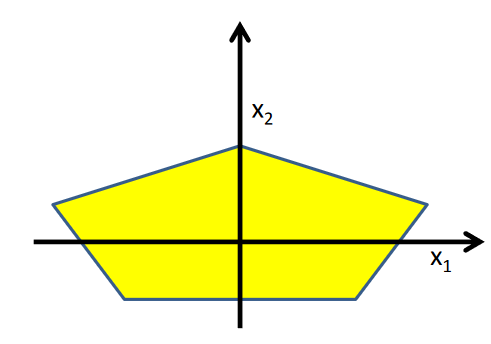
\includegraphics[width=0.5\textwidth]{2_penta_boundary}
\end{figure}

\hfill\break
Recall that should we have pentagonal boundary, that would means that we have boundaries for each sides of the pentagon and the network will fire if the input value exceeds the boundary threshold value. One thing to notice that, only within the pentagon are all five perceptrons going to output $1$. This would imply that the network will fire if \textbf{sum of all of the output} exceeds the \textbf{sum of the threshold boundary value}.

\begin{figure}[H]
	\centering
	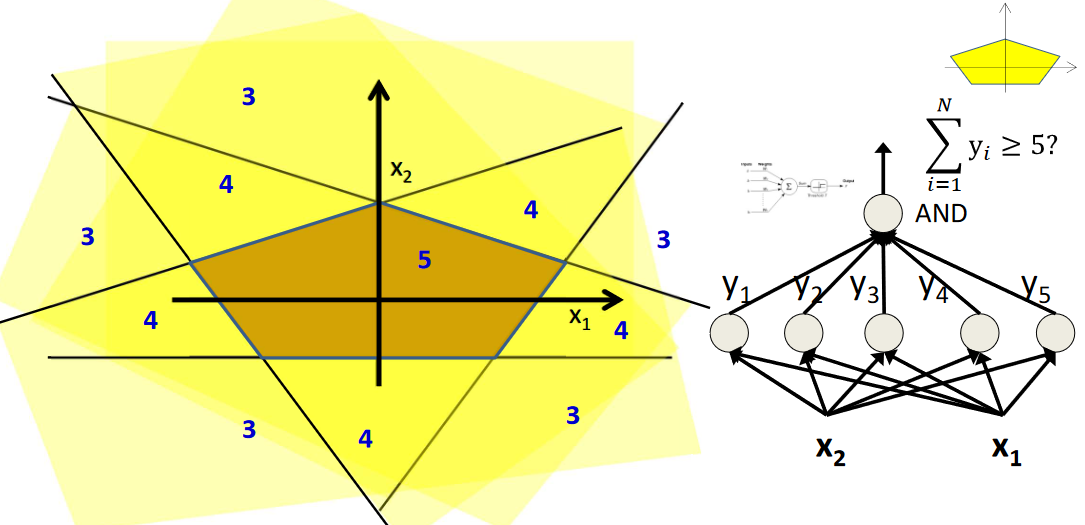
\includegraphics[width=\textwidth]{2_sum_output}
\end{figure}

And if there is more than one closed boundaries, we have to OR them together to get the complex decision boundary. This would means that a third layer would be required.

\begin{figure}[H]
	\centering
	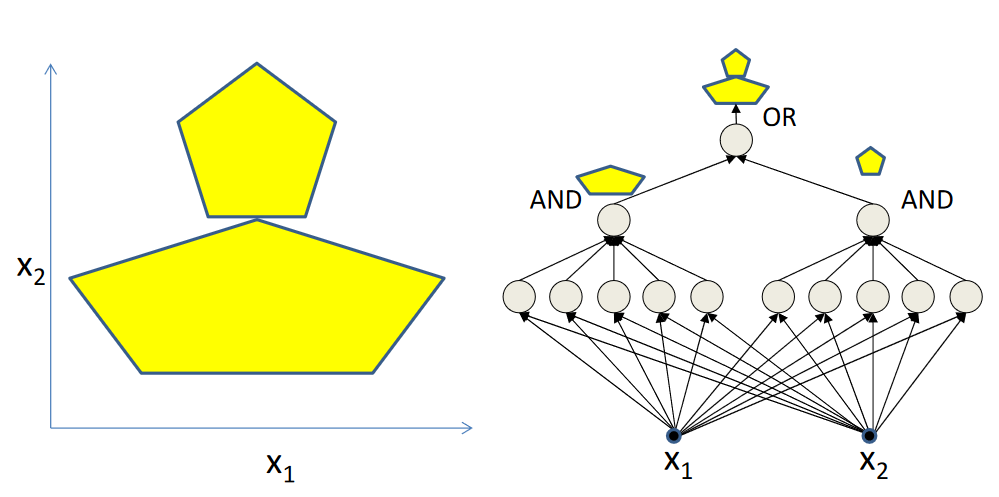
\includegraphics[width=\textwidth]{1_complex}
\end{figure}

The question is, is it possible to compose these decision boundaries with only one hidden layer?

\hfill\break
\textbf{Case: Square boundary}
\\\\
The sum of the output of the inner boundary is 4. Instead of having output layer of AND-ing all of the output of the previous layer perceptron, we just set the threshold value to be the sum of the threshold value of the individual perceptron. The last output neuron is performing SUM instead of AND.

\begin{figure}[H]
	\centering
	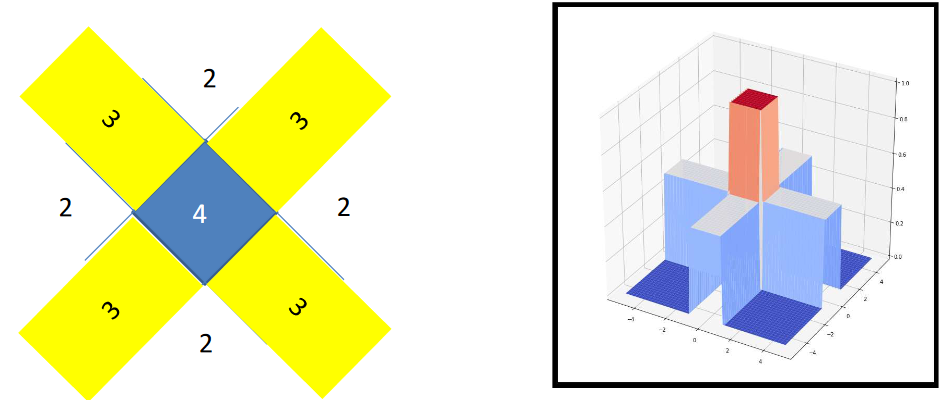
\includegraphics[width=\textwidth]{2_square_boundary}
\end{figure}

\hfill\break
\textbf{Case: Pentagon boundary}

\begin{figure}[h]
	\centering
	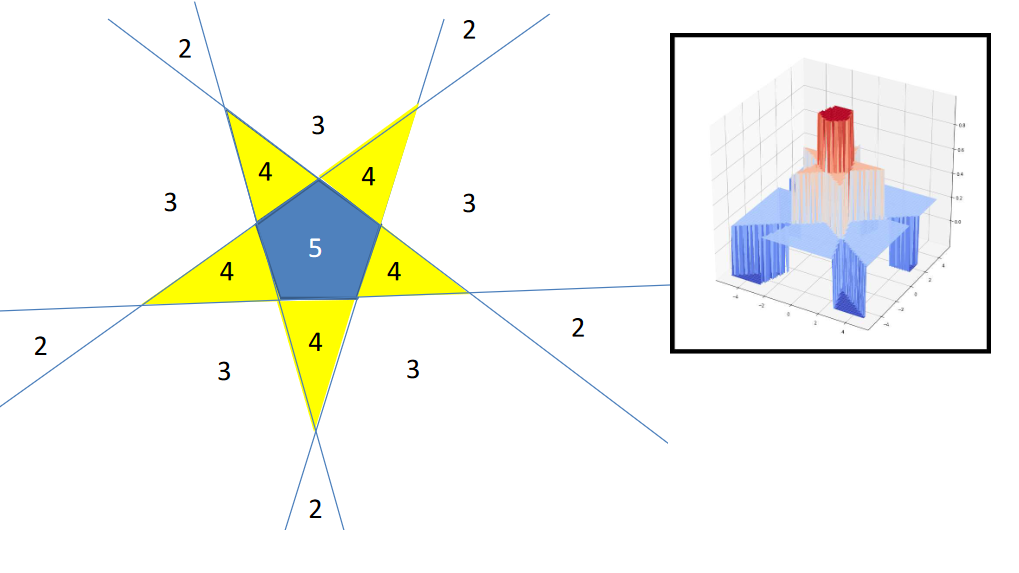
\includegraphics[width=\textwidth]{2_pentagon_boundary}
\end{figure}

\hfill\break
\textbf{Case: Hexagon boundary}

\begin{figure}[H]
	\centering
	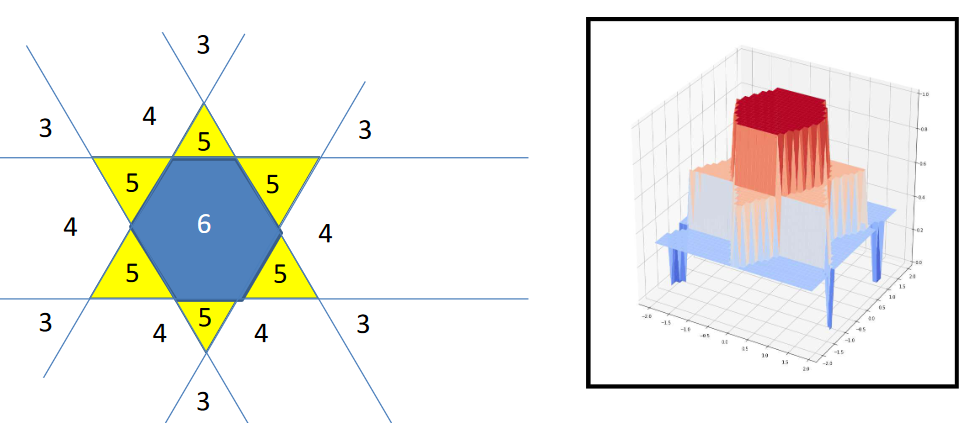
\includegraphics[width=\textwidth]{2_hexagon_boundary}
\end{figure}

\hfill\break
What if we want to compose composite decision boundary with single hidden layer?

\begin{figure}[H]
	\centering
	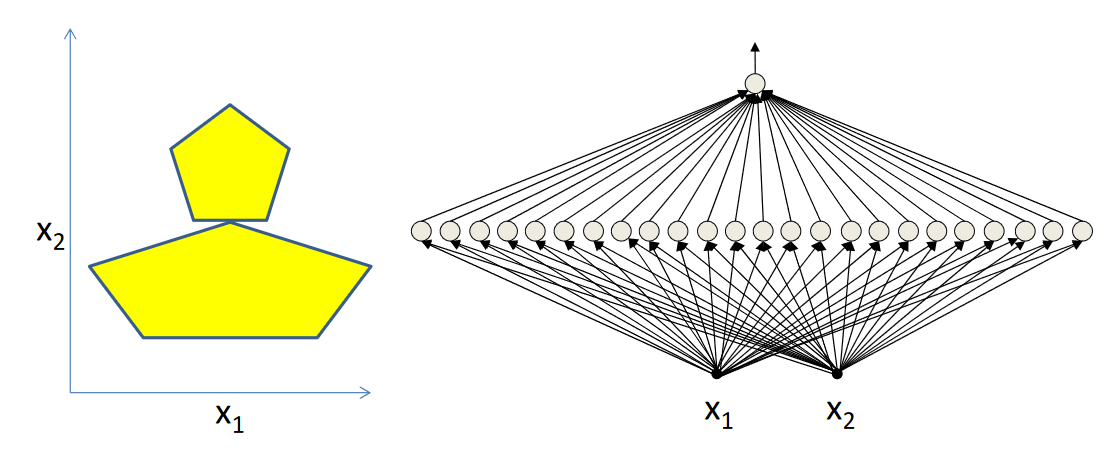
\includegraphics[width=\textwidth]{2_composite_boundary}
\end{figure}

\hfill\linebreak
If we could just somehow finagle these boundaries, it would not be possible because some of the sides of the lower pentagon will intercept with some of the edges of the upper pentagon. So any threshold that can capture lower pentagon will accidentally capture the upper pentagon region that is outside of the region of the lower pentagon.

Consider a square polygon. We would need a network with four neuron in a hidden layer to be able to describe the decision boundary. The threshold value on the side area of the polygon would be 3 and the rest of the area will have threshold value of 2. The same principle will apply to higher dimension polygon where the threshold value would be $s$, $s-1$, $s-2$ $...$ .

We can observe that the first outer layer that is adjacent with the decision boundary would have $s-1$ threshold value. Another observation that could be noticed is that the sum of the area that is outside the decision boundary will always bigger than the sum inside poligon.

\hfill\linebreak
\textbf{Case: Pentagon}

\begin{align*}
	\text{Inner threshold value} &= 5 \\
	\text{Sum of the threshold value of the first outer layer} &= 4 \times 5 \\
	&= 20 \\
	\text{Sum of the threshold value of the second outer layer} &= 3 \times 5 \\
	&= 15 \\
	\text{Sum of the threshold value of the last outer layer} &= 2 \times 5 \\
	&= 10 \\
\end{align*}

\hfill\break
Another observation that could be made is that as the number of the decision boundary increases, the size of the first outer layer will be decreasing. Looking back at the possibility of creating single layer MLP for composite boundary, say if we want to compose a single hidden layer MLP for these outer regions, it would be possible only if the region is really small and does not overlap with the first outer region of another boundary. That being said, constructing MLP for composite boundaries would be possible if these regions are so small that it would not overlap with each other.

\hfill\break
Since for any polygons, the size of the first outer layer will be smaller as the number of sides / decision boundary increases, this would means a circle would have the smallest area of first outer layer since the number of edges $\rightarrow\infty$. Increasing the number of sides will reduces the area outside the polygon that have $\frac{N}{2}<\sum_{i}{y_i}<N$.

\hfill\break
Hypothetically speaking, this would means for a single layer MLP for decision boundary of circle:
\begin{itemize}
	\item The number of neurons will become infinitely large.
	\item Sum of N inside the circle, $\frac{N}{2}$ outside almost everywhere.
\end{itemize}

\begin{figure}[H]
	\centering
	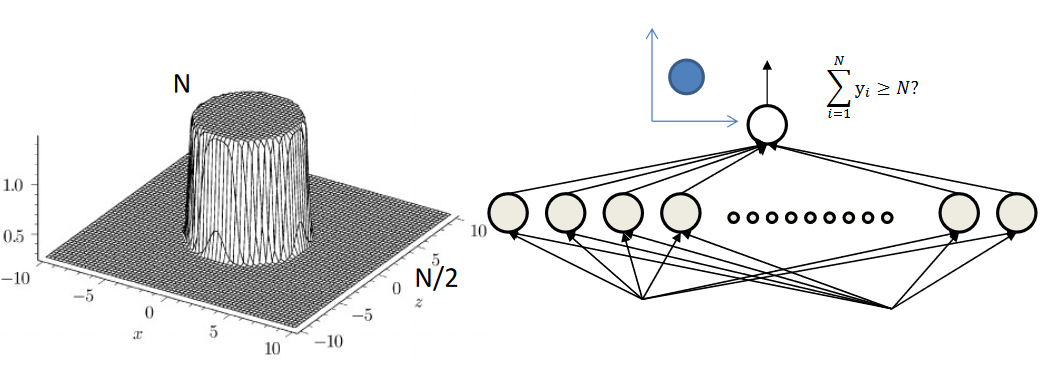
\includegraphics[width=\textwidth]{2_circle_mlp}
\end{figure}

Based on the MLP constructed, if we sum all of these outputs and use a threshold:

\begin{align}
	\sum^N_{i=1}\mathbf{y}_i - \frac{N}{2} \geq 0
\end{align}

\hfill\break
A decision boundary for a perfect circle can be obtained. We also can take a 2 different circle subnets which compose of circles in two different position and still use the same threshold value on the output perceptron. This is because the ``sum'' of two circles of the individual subnets is exactly $\frac{N}{2}$ inside either circle and almost $0$ everywhere outside of the circles.

\begin{figure}[H]
	\centering
	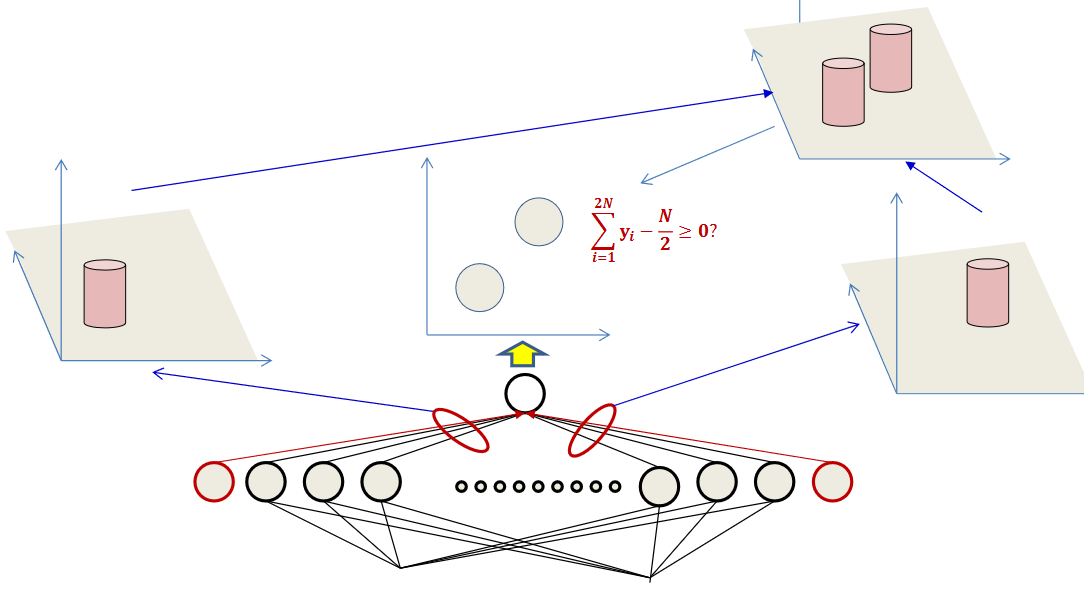
\includegraphics[width=\textwidth]{2_multiple_circles}
\end{figure}

\hfill\break
This would also means that it is possible to use subnets of circle decision boundary to compose any arbitrary figure. We just have have to fill in the composite shapes with enough circle decision boundary. An accurate approximation could be achieved with greater number of smaller circles. This demonstrate the capabilities of one hidden layer MLP being able to model any classification boundary with enough number of neurons.

\begin{figure}[H]
	\centering
	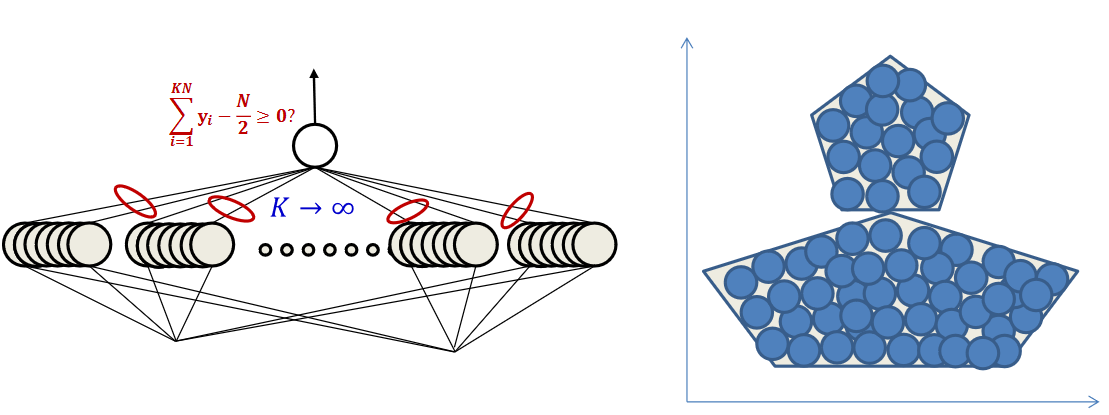
\includegraphics[width=\textwidth]{2_circle_mlp_composite}
\end{figure}

\subsection{Performance comparison between deep network and single layer network.}
 
 \begin{figure}[H]
 	\centering
 	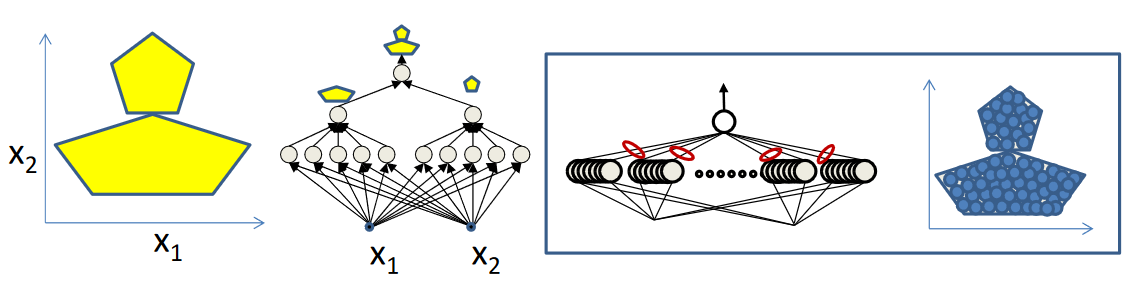
\includegraphics[width=\textwidth]{2_deep_vs_one}
 \end{figure}
 
Deep networks require far fewer neutrons to achieve the same result. Depending on the compleexity of the decision boundary, a naive one-hidden-layer neural network will require infinite hidden neurons. For example, consider an image below, a single layer MLP would require infinite amount of neurons as sum of subset of the circles that is going to be filled into the yellow region.

 \begin{figure}[H]
	\centering
	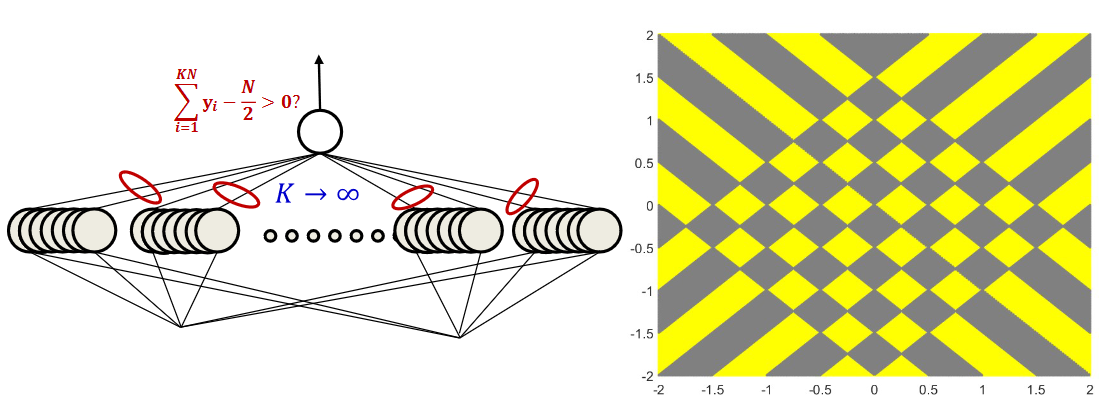
\includegraphics[width=\textwidth]{2_infinite}
\end{figure}

\hfill\break
Howerver, if observed carefully, this image contains 16 lines and 40 segments forming the yellow regions. This would means that we can compose a 2 hidden layer MLP  where every individual neurons on the same layer are XOR-ed together such that

\begin{itemize}
	\item 16 neurons on the first hidden layer.
	\item 40 neurons on the second hidden layer.
	\item 1 neurons on the output layer.
\end{itemize}

 \begin{figure}[H]
	\centering
	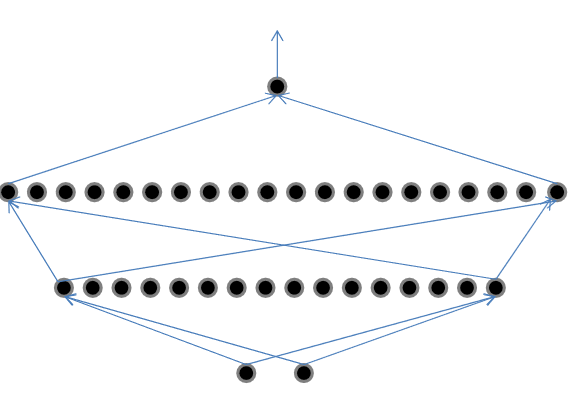
\includegraphics[width=0.5\textwidth]{2_2_layer_mlp}
\end{figure}

\hfill\break
Alternatively, we could observe that the output of the first layer is every 16 individual lines of the decision boundary $Y$, it form a pattern such that for a single neuron that corresponds to each of the line to fire, it is XOR-ed with the rest of the neurons of every other lines. This would mean that the output of the network is:

\begin{align}
	Y_1 \oplus Y_2 \oplus ... \oplus Y_{16}
\end{align}

\hfill\break
This would also means that we can compose the first layer of the network as standard XOR network:

 \begin{figure}[H]
	\centering
	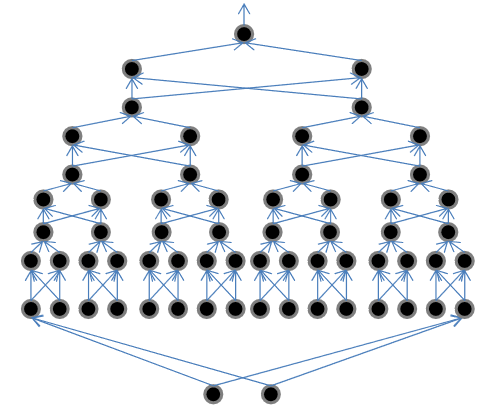
\includegraphics[width=0.5\textwidth]{2_first_layer_xor}
\end{figure}

\hfill\break
The typical XOR network will require $16 + 155\times 3 = 61$ neurons. It is also possible to achieve the network with 46 neurons if we are using two-neurons XOR model. We can summarized that the number of neurons required in shallow network is potentially exponential in the dimensionality of the input. Deeper networks may require far fewer neurons than shallower networks to express the same function, making them much more expressive and smaller than their single layer counterparts.

\subsection{Sufficiency of Architecture.}

A neural network can represent any function provided that it is sufficiently abroad and deep to represent the function, however not all architectures can represent any function. Consider a boundary condition shown below:

 \begin{figure}[H]
	\centering
	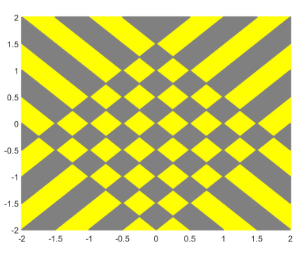
\includegraphics[width=0.5\textwidth]{2_checker_boundary}
\end{figure}

\hfill\break
A network with 16 or more neurons in the first layer is capable of representing the boundary condition perfectly. However, a network that is having less than 16 neurons in the first layer would not be able to represent this pattern exactly. 

 \begin{figure}[H]
	\centering
	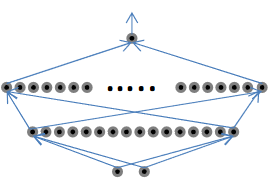
\includegraphics[width=0.5\textwidth]{2_16}
\end{figure}

 \begin{figure}[H]
	\centering
	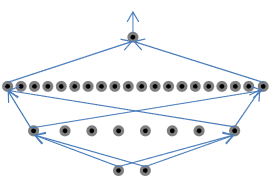
\includegraphics[width=0.5\textwidth]{2_not_16}
\end{figure}

\hfill\break
This is because a network with $x$ threshold neurons in the first layer may only capture $x$ number of boundaries. This gives information about which boundary where the threshold is applied to, but not where the boundary is. Similarly restriction is also applied to the higher layers. A 2-layer network with 16 neurons in the first layer alone are not sufficient to represent the checkered region of the pattern if the second layer is having less than 40 neurons inside it. Regardless of depth, every layer must be sufficiently wide in order to express the function accurately.
\\\\
This is because we are using the threshold activation value. It gates information in the input from the later layer since the output is either $0$ or $1$. This will lead to a pattern of outputs within any region is identical while the subsequent layers do not obtain enough information to partition them. In order to maintain the position information such as the distance from a boundary, a continuous activation function such as sigmoid function has to be used.

\begin{figure}[H]
	\centering
	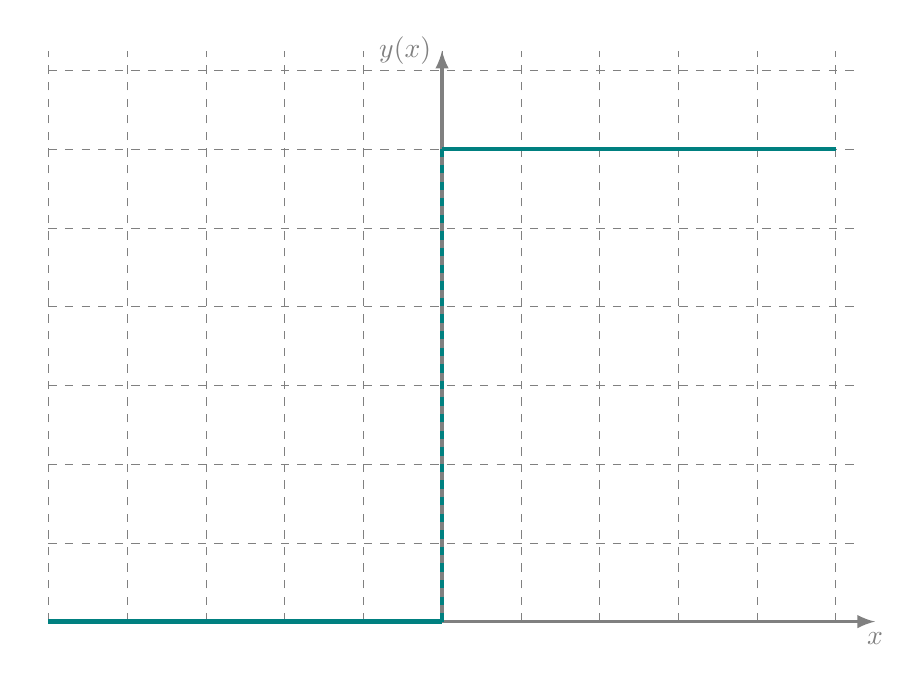
\begin{tikzpicture}
		% grid
		\draw[help lines,dashed] (0,0) grid (10.25, 7.25);
		
		% Axes
		\draw[very thick,-latex, gray] (0,0) -- (10.5,0) 
		node[below]{$x$};
		
		\draw[very thick,-latex, gray] (5,0) -- (5,7.25) 
		node[left]{$y(x)$};
		
		\draw[ultra thick,teal] (0,0) node[left,black](s0){$$}
		
		plot[domain=0:5,
		samples = 50,
		smooth]({\x}, {0})
		
		
		plot[domain=5:10,
		samples = 50,
		smooth]({\x}, {6});
		
		\draw[dashed, ultra thick, teal] (5,0) -- (5,6);
		
	\end{tikzpicture}
\end{figure}

\hfill\break
This activation function caused a well defined boundary limit which lead to the following pattern.

\begin{figure}[H]
	\centering
	\begin{tikzpicture}
		\begin{axis}[
			width=11.25cm,
			height=11.25cm,
			axis lines = middle,
			grid=both,
			xlabel = {$x$},
			ylabel = {$y$},
			xmin=-10, xmax=10,
			ymin=-10, ymax=10]
			every axis plot/.append style={ultra thick},
		
			\addplot [name path = A,
			-latex,
			domain = -10:12,
			samples = 1000] {x + 7} 
			node [very near end, right] {$$};
			
			\addplot [name path = B,
			-latex,
			domain = -10:12,
			samples = 1000] {x + 3} 
			node [very near end, right] {$$};
			
			\addplot [name path = C,
			-latex,
			domain = -10:12,
			samples = 1000] {x + -1} 
			node [very near end, right] {$$};
			
			\addplot [name path = D,
			-latex,
			domain = -10:12,
			samples = 1000] {x + -5} 
			node [very near end, right] {$$};
			
			\addplot [teal, opacity=0.4] fill between [of = A and B, soft clip={domain=-10:12}];
			\addplot [yellow, opacity=0.4] fill between [of = B and C, soft clip={domain=-10:12}];
			\addplot [magenta, opacity=0.4] fill between [of = C and D, soft clip={domain=-10:12}];
			
		\end{axis}
	\end{tikzpicture}
\end{figure}

\hfill\break
A continuous activation functions result in graded output at the layer. The gradation provides information to subsequent layers, to capture information ``missed'' by the lower layer. This would also means that, if the network is not having sufficient number of neurons, we are still having information regarding inputs that has not crossed the threshold value but were pretty close with the boundary. 

\begin{figure}[H]
	\centering
	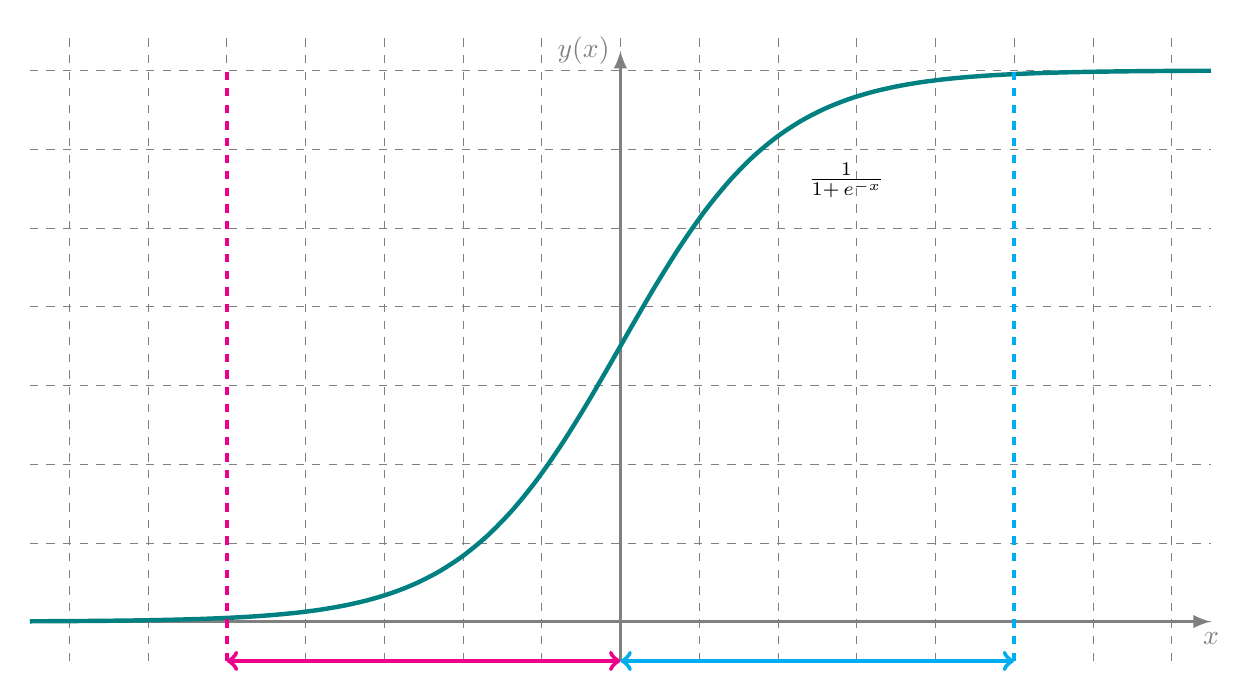
\begin{tikzpicture}
		% grid
		\draw[help lines,dashed] (-7.5,-.5) grid (7.5, 7.5);
		
		% Axes
		\draw[very thick,-latex, gray] (-7.5,0) -- (7.5,0) 
		node[below]{$x$};
		
		\draw[very thick,-latex, gray] (0,-.5) -- (0,7.25) 
		node[left]{$y(x)$};
		
		\draw[ultra thick,teal] (3.5, 5.6) node[left,black](s0){$\frac{1}{1 +\,e^{-x}}$}
		plot[domain=-7.5:7.5,
		samples = 50,
		smooth]({\x}, {7/(1 + exp(-1 * \x))});
		
		\draw[dashed, ultra thick, magenta] (-5,-.5) -- (-5,7);
		\draw[dashed, ultra thick, cyan] (5,-.5) -- (5,7);
		
		\draw[<->, ultra thick, magenta] (-5,-.5) -- (0,-.5);
		\draw[<->, ultra thick, cyan] (-0,-.5) -- (5,-.5);
		
	\end{tikzpicture}
\end{figure}

\hfill\break
However, a continuous function such as sigmoid function also comes with several drawbacks. Beyond the certain $x$ values, the activation function is behaving as a step function. So there is possibility that the information of the data might be loss if the input value is outside the range of the sigmoid function that behave as a continuous function. 
\\\\
We want to have an activation function that continuous to give information from the boundary regardless of how far away the input from the boundary value. Activation functions with more gradation such as softplus or ReLU able to pass information when there is not enough neurons to describe the boundary solution. 

\begin{figure}[H]
	\centering
	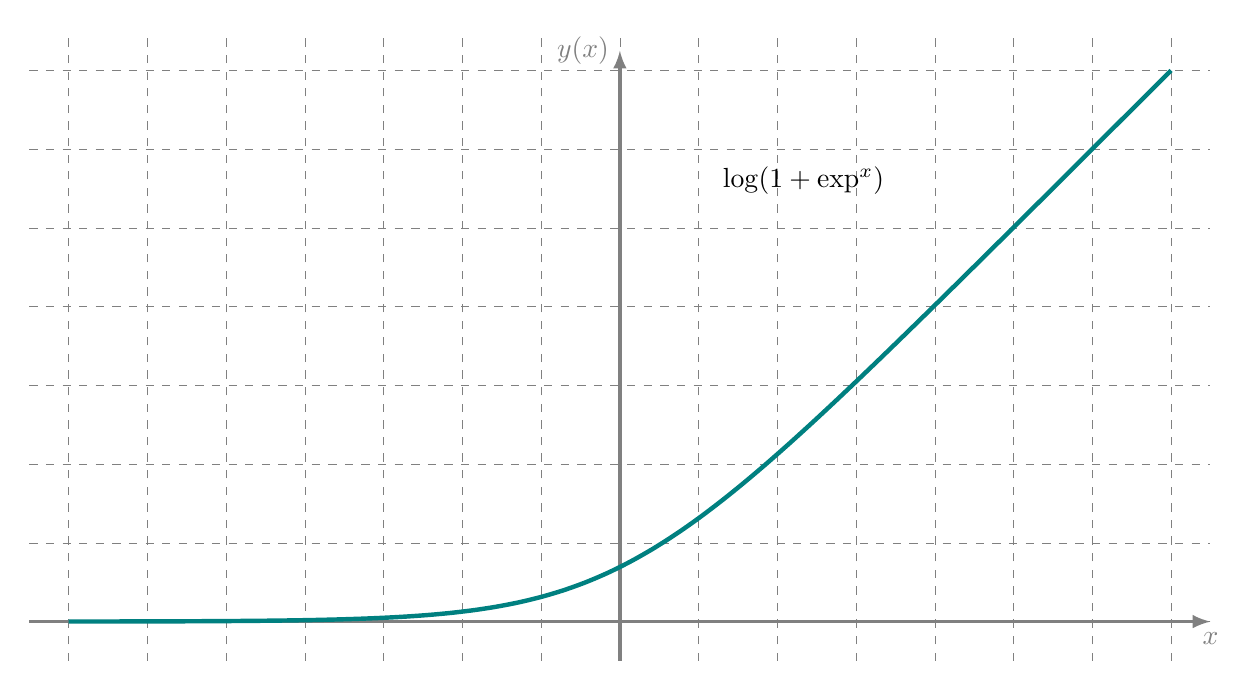
\begin{tikzpicture}
		% grid
		\draw[help lines,dashed] (-7.5,-.5) grid (7.5, 7.5);
		
		% Axes
		\draw[very thick,-latex, gray] (-7.5,0) -- (7.5,0) 
		node[below]{$x$};
		
		\draw[very thick,-latex, gray] (0,-.5) -- (0,7.25) 
		node[left]{$y(x)$};
		
		\draw[ultra thick,teal] (3.5, 5.6) node[left,black](s0){$\log (1 + \exp^{x})$}
		plot[domain=-7:7,
		samples = 50,
		smooth]({\x}, {ln(1 + e^\x))});
	\end{tikzpicture}
\end{figure}

\begin{figure}[H]
	\centering
	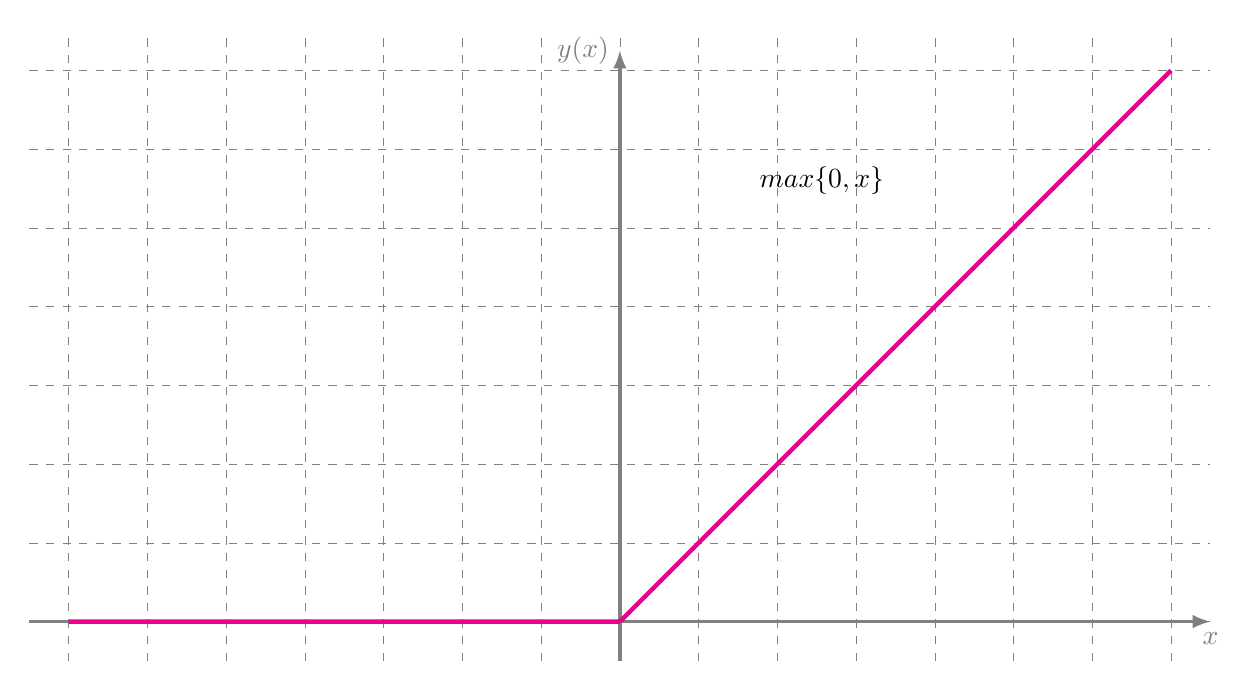
\begin{tikzpicture}
		% grid
		\draw[help lines,dashed] (-7.5,-.5) grid (7.5, 7.5);
		
		% Axes
		\draw[very thick,-latex, gray] (-7.5,0) -- (7.5,0) 
		node[below]{$x$};
		
		\draw[very thick,-latex, gray] (0,-.5) -- (0,7.25) 
		node[left]{$y(x)$};
		
		\draw[ultra thick,magenta] (3.5, 5.6) node[left,black](s0){$max\{0,x\}$}
		plot[domain=0:7,
		samples = 50,
		smooth]({\x}, {\x})
		(-7,0) -- (0,0);
	\end{tikzpicture}
\end{figure}

\subsection{Width vs Activation Function vs Depth}
\begin{itemize}
	\item Narrow layers can still pass information to subsequent layers if the activation function is sufficiently graded.
	\item However, this will require the network to have greater depth to permit subsequent layers to capture the patterns.
	\item Care to be taken when implementing the activation function to ensure its non-linearity to prevent the the output from collapsing.
\end{itemize}












